\begin{frame}{Introduction}
\begin{center}
\begin{itemize}
    \item \textbf{Reference Genes (RG)} 
    \begin{itemize}
        \item Constitutive genes
        \vspace{3pt}
        \item Expressed in all cells
        \vspace{3pt}
        \item Used in internal controls (gene expression analysis)
    \end{itemize}
\end{itemize}
\vspace{5pt}
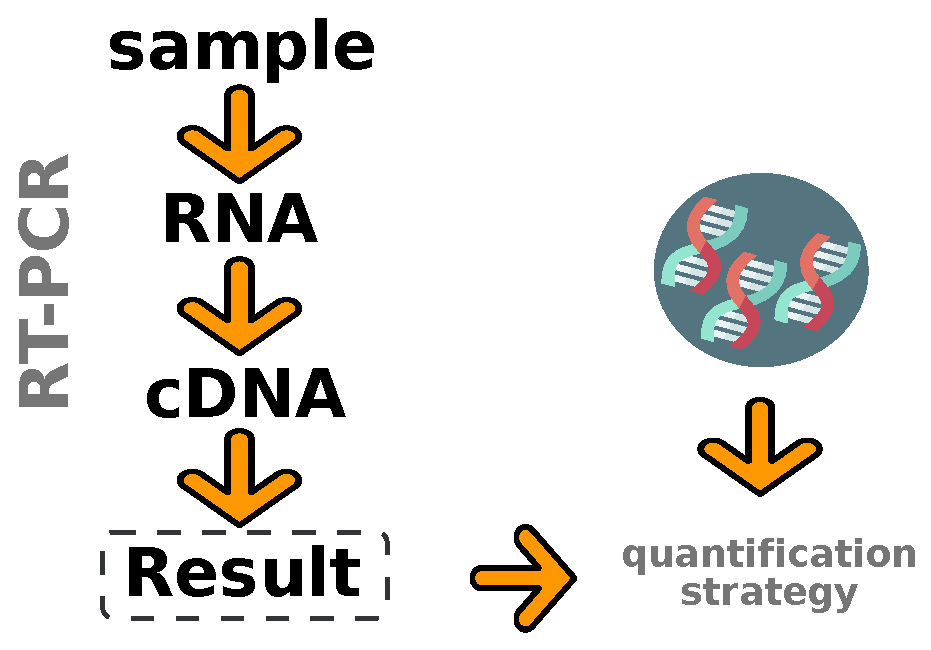
\includegraphics[scale=.3]{figures/rt_pcr.eps}
%Reference gene must in turn demonstrate the variability resulting from imperfections of the technology used and preparatory procedures—this ensures that any variation in the amount of genetic material will relate to the same extent as the object of research and control.
%para normalizar la expresión génica
%-Los genes de referencia en Quantitative RT-PCR sirven para normalizar los datos, debido a que los GR tienen un minimo cambio de su expresión genética en diferentes condiciones de estrés. El gen de referencia a su vez debe demostrar la variabilidad resultante de las imperfecciones de la tecnología utilizada y los procedimientos preparatorios, esto asegura que cualquier variación en la cantidad de material genético se relacione en la misma medida que el objeto de investigación y el de control (gen de referencia).
\begin{itemize}
    \item Normalize gene expression
    \item Demonstrates the variability and imperfections of the technology
\end{itemize}

\end{center}
\end{frame}

%#################################################
%----------------- Second frame ------------------
%#################################################
%Based on optimziation algorithms: minimum cost network flow problem
\begin{frame}{Introduction}
\Large\textcolor{dodgerblue}{\textbf{Identify candidates for Reference Genes}}
\vspace{5pt}
\begin{center}
\begin{itemize}
    \normalsize
    \item Pipeline:
\end{itemize}
\vspace{13pt}
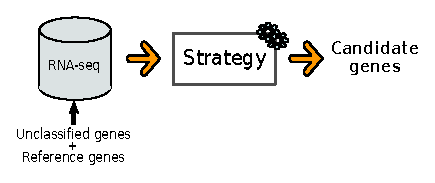
\includegraphics[scale=1.3]{figures/strategy.eps}
\vspace{18pt}
\begin{itemize}
    \normalsize
    \item Strategies
    \begin{itemize}
        \item Based on clustering (Euclidean distance)
        \vspace{3pt}
        \item Based on optimization algorithms
\end{itemize}
\end{itemize}
\end{center}
\end{frame}
